\scanpage{32}
\diagram{\begin{tikzcd}[ampersand replacement=\&,column sep=.48em,row sep=1.4em]
\& \& {D^{012}=A^{\vcenter{\hbox{\tikz[scale=.11]{\draw[->](0,0)--(0,1.4);\draw[->](0,0)--(1.6,0);}}}}}\arrow[dll]\arrow[dl]\arrow[d]\arrow[dr]\arrow[drr,very thick] \& \& \\
\widetilde S\arrow[d] \& {\substack{\vec A\\\shortparallel\\D^{01}}}\arrow[dl]\arrow[dr] \& \widetilde A\arrow[d] \& {\substack{A^\uparrow\\\shortparallel\\D^{12}}}\arrow[dl]\arrow[dr] \& \widetilde F\arrow[d]\\
{\substack{S\\ \shortparallel\\D^0}} \& \& {\substack{A\\ \shortparallel\\D^1}} \& \& {\substack{F\\ \shortparallel\\D^2}}
\end{tikzcd}\qquad
\begin{tikzcd}[ampersand replacement=\&,column sep=.35em,row sep=1.4em]
\& {A^{\vcenter{\hbox{\tikz[scale=.11]{\draw[->](0,0)--(0,1.4);\draw[->](0,0)--(1.6,0);}}}}=D^{012}}\arrow[d] \& \\
\& {\substack{A^\wedge\\\shortparallel\\D^{02}}}\arrow[dl]\arrow[dr] \& \\
{\substack{S\\ \shortparallel\\D^0}} \& \& {\substack{F\\ \shortparallel\\D^2}}
\end{tikzcd}}

Icosaèdre gauche (sommets $S$ etc\ldots) en termes de $(E,\omega)$, $E$ ens \unsure{à|:} $5$ éléments, $\omega$ une orientation

\diagram{$\begin{array}{ll}
S\simeq\mathrm{Pent}_\omega(E)&\text{struct. pent. comp. avec }\omega\\
A\simeq\deleted{\unsure{\mathscr P}}\mathrm{Car}(E)&\shortstack[l]{partitions de degrés $(2,2,1)$\\$\simeq$ structures carrées sur une partie de $E$}\\
F\simeq\deleted{\unsure{\mathscr P_3|\mathfrak P_3}}\mathrm{Tr}_3(E)&\shortstack[l]{\deleted{parties à $3$ él.}\\triangles $\subset E$}\\
\vec A\simeq\mathrm{Pent}^s_\omega(E)&\shortstack[l]{$\omega$-structures pentagonales à somm.\\marqué}\\
A^\uparrow\simeq\deleted{\unsure{\mathscr P_3|\mathfrak P_3}}\unsure{\dot{\mathrm{Tr}}_3|\mathrm{Tr}_3}(E)&\text{\deleted{parties à trois él.} \inserted{triangles} ponctués}\\
A^\wedge\simeq\mathrm{Pent}^a_\omega(E)&\text{structure pent. à arête marquée}\\
\hfill\shortparallel\hfill&\\[-3pt]
\hfill\mathrm{Pent}^s_\omega(E)\hfill&\\
A^{\vcenter{\hbox{\tikz[scale=.11]{\draw[->](0,0)--(0,1.4);\draw[->](0,0)--(1.6,0);}}}}\simeq\mathrm{Rep}_\omega(E)&\shortstack[l]{ordres totaux\\sur $E$ comp.\\avec $\omega$}
\end{array}$}

\figure{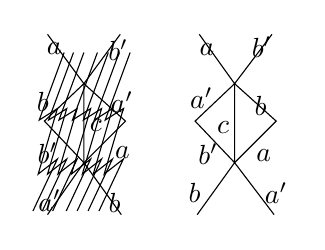
\begin{tikzpicture}[scale=.66,baseline]
\draw(-.7,1.85)--(0,.9)--(.8,.18)--(0,-.62)--(-.76,.18)--(0,.9)--(.7,1.85);
\draw(0,.9)--(0,-.62)--(-.7,-1.62) (0,-.62)--(.72,-1.62);
\node at(-.57,1.57){$\deleted{a}$};\node at(.66,1.55){$\deleted{b'}$};
\node at(-.79,.54){$\deleted{b}$};\node at(.73,.55){$\deleted{a'}$};
\node at(.23,.1){$\deleted{c}$};\node at(-.70,-.43){$\deleted{b'}$};\node at(.74,-.43){$\deleted{a}$};
\node at(-.66,-1.35){$\deleted{a'}$};\node at(.59,-1.39){$\deleted{b}$};
\foreach \x in {-.76,-.58,-.38,-.12,.09,.30,.51}{\draw[thin](\x-.22,-1.55)--(\x+.25,-.55)--(\x-.12,-.84)--(\x+.25,.42)--(\x-.1,.2)--(\x+.38,1.5);}
\begin{scope}[xshift=2.9cm]
\draw(-.68,1.85)--(0,.9)--(.8,.18)--(0,-.62)--(-.76,.18)--(0,.9)--(.72,1.85);
\draw(0,.9)--(0,-.62)--(-.72,-1.62) (0,-.62)--(.76,-1.62);
\node at(-.53,1.56){$a$};\node at(.52,1.60){$b'$};\node at(-.64,.62){$a'$};\node at(.5,.48){$b$};
\node at(-.22,.06){$c$};\node at(-.51,-.45){$b'$};\node at(.56,-.49){$a$};\node at(-.77,-1.21){$b$};\node at(.8,-1.21){$a'$};
\end{scope}
\end{tikzpicture}}

\figure{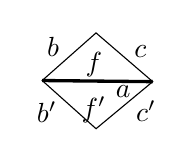
\begin{tikzpicture}[scale=.72]
\draw(-.95,.12)--(0,.96)--(1,.10)--(0,-.73)--cycle;
\draw[very thick](-.95,.12)--(1,.10);
\node at(-.76,.72){$b$};\node at(.78,.64){$c$};\node at(-.04,.40){$f$};\node at(.48,-.08){$a$};
\node at(-.04,-.40){$f'$};\node at(-.87,-.43){$b'$};\node at(.88,-.42){$c'$};
\end{tikzpicture}\qquad
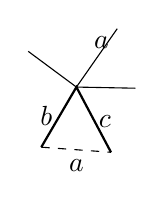
\begin{tikzpicture}[scale=.72]
\draw(-.85,.95)--(0,.32)--(.72,1.35) (0,.32)--(1.04,.30);
\draw[thick](-.62,-.74)--(0,.32)--(.61,-.83);\draw[dashed](-.62,-.74)--(.61,-.83);
\node at(.44,1.10){$a$};\node at(-.53,-.19){$b$};\node at(.50,-.28){$c$};\node[below]at(0,-.79){$a$};
\end{tikzpicture}}

\diagram{$\begin{array}{ll}
\widetilde S\simeq\deleted{\unsure{\mathrm{Pent}_\omega(E)}}\overrightarrow{\mathrm{Pent}}_\omega(E)&\shortstack[l]{permutations circulaires comp.\\avec $\omega$}\\
\widetilde A\simeq\overrightarrow{\mathrm{Car}}(E)&\text{carrés orientés }\subset E\\
\widetilde F\simeq\deleted{\unsure{\mathscr P_3|\mathfrak P_3}}\overrightarrow{\mathrm{Tr}}_3(E)&\shortstack[l]{triangles orientés $\subset E$\\\deleted{parties à trois él. avec ordre circ. dessus}}
\end{array}$}

\[
\left\{\begin{aligned}
\sigma_0(a_1,\underline{a_2,a_3,a_4,a_5})&=(a_1,a_4,a_5,a_2,a_3)\\
\sigma_1(a_1,a_2,a_3,a_4,a_5)&=(a_2,a_1,a_5,a_4,a_3)\\
\sigma_2(a_1,a_2,a_3,a_4,a_5)&=(a_1,a_5,a_4,a_3,a_2)
\end{aligned}\right.
\]
\figure{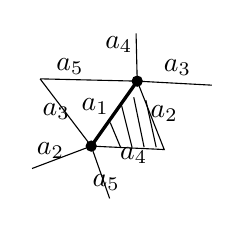
\begin{tikzpicture}[scale=.73]
\coordinate(p)at(-.56,-.37);\coordinate(q)at(.24,.76);\coordinate(r)at(.71,-.43);\coordinate(l)at(-1.45,.80);
\draw(l)--(q)--(1.54,.69) (q)--(.22,1.59) (l)--(p)--(r)--(q) (-1.59,-.76)--(p)--(-.24,-1.28);
\draw[very thick](p)--(q);\fill(p)circle(2.8pt) (q)circle(2.8pt);
\foreach \x/\y in {-.23/.04,-.03/.33,.18/.48,.39/.43}{\draw[thin](\x,\y)--(\x+.18,-.39);}
\node at(-.49,.32){$a_1$};\node at(.71,.20){$a_2$};\node at(.18,-.54){$a_4$};
\node at(-1.17,.23){$a_3$};\node at(-1.27,-.44){$a_2$};\node at(-.30,-1.01){$a_5$};
\node at(-.93,1.02){$a_5$};\node at(-.08,1.39){$a_4$};\node at(.94,1.00){$a_3$};
\end{tikzpicture}}
% archive sheet number: 31
